\section{Classification binaire}
La classification binaire est un  problème consistant à prendre un vecteur de caractéristiques \textbf{x} et à décider de laquelle des deux étiquettes (ou classes) il appartient. Par exemple  on peut prendre un vecteur de caractéristiques contenant la taille et le poids d'une personne et essayer de prédire  le sexe de la personne.Il existe de nombreux algorithmes qui traitent ce problème, notamment la régression logistique, les machines à vecteurs de support, etc.
Dans cette section, nous examinerons la discrimination linéaire de Fisher, qui est une technique permettant d'effectuer une classification binaire lorsque les caractéristiques sont des quantités continues.\\
L'analyse discriminante linéaire de Fisher aborde le problème de la classification en trouvant un vecteur \textbf{w} sur lequel
nous pouvons projeter les données sur un vecteur tel qu'il est plus facile de définir un point qui sépare les deux classes avec une grande marge. Pour ce faire, nous choisissons un vecteur w qui maximise le rapport entre les variances interclasse et intraclasse. Intuitivement, cela a du sens car nous voulons maximiser la séparation entre les différentes classes, tout en minimisant la séparation au sein de chaque classe. Une fois que nous avons ce vecteur \textbf{w}, nous pouvons classifier un point de données x en calculant $\textbf{w}^\intercal \mathbf{x}$ et en le comparant au seuil c correspondant à notre point de séparation.\\
\begin{figure}[h]
    \centeryy ning
    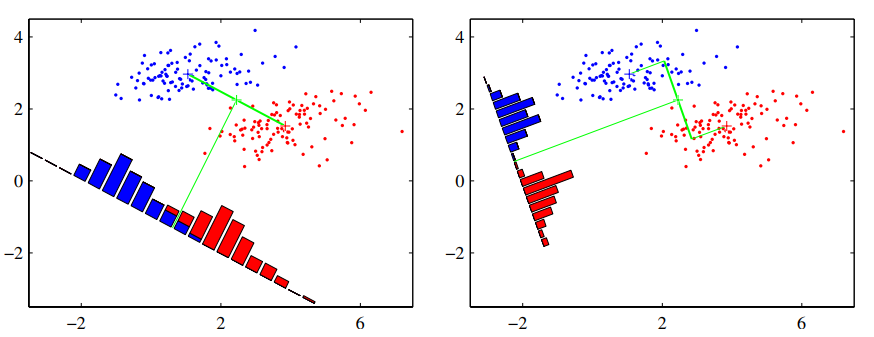
\includegraphics[width=1\textwidth]{1.PNG}

    \label{fig:figure 1}
\end{figure}\\

\\
De manière plus formelle,onsidérons un problème à deux classes dans lequel il y a N{_1}$  points de la classe C{_1}$  et N{_2}$  points de la classe C{_2}$ , de sorte que les vecteurs moyens des deux classes sont donnés par:
\begin{equation}
 u{_1}={\frac {1}{N{_1}}}\sum _{i=1}^{n}X_{i} ,  et    u{_2}={\frac {1}{N{_2}}}\sum _{i=1}^{n}X_{i}
\end{equation}
La mesure la plus simple de la séparation des classes, lorsqu'elle est projetée sur \mathbf{w}, est la
séparation des moyennes des classes projetées. Ceci suggère que nous pourrions choisir \mathbf{w} de manière à
maximiser
\begin{center}
  \begin{equation}
    u{_2}-u{_1}=\textbf{w}^\intercal (u{_2} -u{_1})

  \end{equation}
  \begin{equation}
    u{_k}=\textbf{w}^\intercal (u{_k})

  \end{equation}
\end{center}
La variance intra-classe des données transformées de la classe C{_k} $ est donc donnée par
\begin{center}
  \begin{equation}
    \sigma{_k}^2=\sum_{n \in C{_k}} (Y{_n}-u{_k})
  \end{equation}
\end{center}

où
\begin{equation}
  Y{_n}  = \textbf{w}^\intercal x{_n}
\end{equation}
 Nous pouvons définir la variance intra-classe totale pour l'ensemble des données comme étant simplement $\sigma{_1}^2$+$\sigma{_2}^2$. Le critère de Fisher est défini comme étant le rapport entre la variance interclasse et la variance interne à la classe et est donné par:\\
 \begin{equation}
   \begin{split}
     S  =\frac{\sigma^2{_(intra)}}{\sigma^2{_(extra)}}  \\  =\frac{(u{_2} -u{_1})^2}{\sigma{_1}^2+\sigma{_2}^2} \\  =\frac{(\textbf{w}^\intercal (u{_2} -u{_1}))^2}
     {
     (\sum_{i ,c{_i}=1}(\textbf{w}^\intercal(x{_i} -u{_1})))^2+ (\sum_{i ,c{_i}=2}(\textbf{w}^\intercal(x{_i} -u{_2})))^2
     } \\  =\frac{\textbf{w}^\intercal \mathbf{S{_B}}\mathbf{w}}{\textbf{w}^\intercal \mathbf{S}{_W}\mathbf{w}}
   \end{split}

 \end{equation}
 où $\mathbf{S{_B}}$ est la matrice de covariance entre les deux classes C{_1} $ et {C_2} $ avec \\
 \begin{equation}
   \mathbf{S{_B}}=(u{_2}-u{_1})(u{_2}-u{_1})^\intercal
 \end{equation}
 et $\mathbf{S{_W}}$ la matrice de covariance intra-classe avec
 \begin{equation}
   \mathbf{S}{_W} =\sum_{i ,c{_i}=1}(x{_i}-u{_1})(x{_i}-u{_1})^\intercal +  \sum_{i ,c{_i}=2}(x{_i}-u{_2})(x{_i}-u{_2})^\intercal
 \end{equation}
 En suivant la présentation de \cite{7}, nous pouvons deriver  par rapport à w pour obtenir
 \begin{equation}
   \frac{\partial{S}}{\partial{w}}=0 \Rightarrow (\textbf{w}^\intercal \mathbf{S{_B}}\mathbf{w})\mathbf{S}{_W}\mathbf{w}= (\textbf{w}^\intercal \mathbf{S}{_W}\mathbf{w})\mathbf{S{_B}}\mathbf{w}
 \end{equation}
 $\mathbf{S{_B}} \mathbf{w} $  est dans la même direction que  u{_2}$ -u{_1}$ et que $(\textbf{w}^\intercal \mathbf{S{_B}}\mathbf{w}) $ et  $(\textbf{w}^\intercal \mathbf{S}{_W}\mathbf{w})$ sont des constantes.
Puisque nous ne nous intéressons qu'à la direction et non au facteur  de $\mathbf{w}$, nous pouvons eliminer  les constantes et multiplier les deux côtés par  $\mathbf{S}{_W}^{-1}$ pour obtenir une solution optimale de w
\begin{center}
  $\mathbf{w}^{*}$ $\propto$  $\mathbf{S}{_W}^{-1}$(u{_2} $-u{_1} $)
\end{center}
Une fois que le $\mathbf{w }$ optimale calculé ,nous devons  trouver un seuil de classification c. D'habitude c est pris comme etant le  point médian entre les deux moyennes dans la direction donnée par $\mathbf{w}^{*}$.
\begin{equation}
     c = \frac{\textbf{w}^{*}^\intercal(u{_2}-u{_1})}{2}
\end{equation}
Ainsi, étant donné un point x, on calcule $\textbf{w}^{*}^\intercal$x et on classe  x selon que cette valeur est supérieure ou inférieure à c (seuil).

\section{Classification naïve bayésienne}
Un classificateur Naïve Bayes est une méthode pour classer des vecteurs  caractéristiques à valeur discrète. En particulier, étant donné un vecteur de données x $\in$  $\{1, ...K\}^n$, où K est le nombre de valeurs possibles pour chaque variable
 caractéristique et D est le nombre de variable caractéristiques. Cela nous permet d'écrire la densité conditionnelle de classe comme suit :
 \begin{equation}
    P(\mathbf{x} \mid C=c) =   \prod_{j=1}^D P(\mathbf{x}{_j} \mid C=c)
 \end{equation}
 Les classificateurs de Naïve Bayes sont qualifiés de ``naïves'' car ils supposent l'indépendance des variables ,ce qui est rarement le cas .Malgré cela , ils donnent parfois de bon résultat \cite{8}\\
 Comme son nom l'indique, les classificateurs Naïve Bayes constituent une autre façon d'aborder le problème de la classification.
Si nous avons K classes possibles, alors le modèle se compose de  classe de probabilité  à pirori $\{Pr(C = ci)\}_{i=1}^K$ (c'est-à-dire la probabilité à priori de la classe c{_i} $) et des densités conditionnelles de classe  $\{P(X = x | C = ci)\}_{i=1}^K$, c'est-à-dire la probabilité qu'un objet de la classe c{_i}$ possède un ensemble  de variables  caractéristiques  x.\\
À titre d'exemple , supposons que nous ayons une liste de maladies $\{m{_1}, ..., m{_n}\} $ et un vecteur de symptômes $(s{_1}, ..., s{_m})$  où s{_i}$=1 si la personne présente le symptôme i et 0 si elle ne le présente pas. Le modèle de Naïve Bayes spécifie P(s{_i} = 1 | m{_j}$) $\forall i,j $ (c'est-à-dire la probabilité qu'une personne présente le symptôme i étant donné qu'elle est atteinte de la maladie j) et P(m{_j} $ ) $\forall j $ (c'est-à-dire la probabilité qu'une personne soit atteinte de la maladie j). Ensuite, pour calculer la probabilité qu'une personne atteinte d'une maladie m{_k} $ présente un ensemble particulier de symptômes  $\(s'{_1}, ..., s'{_m}\)$, on calcule
\begin{center}
  P((s'{_1}, ..., s'{_m}) \mid m{_k} ) =   \prod_{j=1}^m P(s{_i}$  =s'{_i}$ \mid m{_k})

\end{center}
Avec ce modèle, la classification fonctionne alors en utilisant une règle de décision à posteriori maximale. Étant donné un point de données x, nous calculons la probabilité postérieure de son appartenance à chaque classe c{_i}$  et classons x dans la classe ayant la probabilité postérieure la plus élevée. Plus précisément, nous calculons.
\begin{equation}
\begin{split}
c^{*}=\DeclareMathOperator{\argmax}{arg\,max}_{i\in {1,....k}}P(C=c{_i} \midX=x)\\
=\DeclareMathOperator{\argmax}{arg\,max}_{i\in {1,....k}}\frac{P(X=x \mid C=c{_i})P(C=c{_i})}{P(X=x)}\\
=\DeclareMathOperator{\argmax}{arg\,max}_{i\in {1,....k}}P(X=x \mid C=c{_i}) P(C=c{_i})

\end{split}
\end{equation}
\\

Notez que dans la dernière étape, puisque P(X = x) est une constante pour toutes les classes le probléme se raméne alors à chercher des numeratuers  . Comme nous le verrons plus tard, le fait de ne pas avoir cette étape de division rend un classificateur de Naïve Bayes plus facile à mettre en œuvre sur un schéma de chiffrement partiellement  homomorphe.

\section{Regression linéaire}
La régression linéaire est l'un des algorithmes  de machine learning les plus fondamentaux .Nous modélisons une variable cible ou de sortie comme une fonction linéaire de variables d'entrée (qui ont vraisemblablement une certaine relation avec la variable cible), plus un terme d'erreur normalement distribué,formellement
\begin{equation}
  y= \langle \beta , \mathbf{x} \rangle +\epsilon
\end{equation}
Par exemple, nous pouvons modéliser l'espérance de vie d'une personne comme une fonction linéaire de son revenu et de son état de santé, donc si nous avons un vecteur x = (revenu, état de santé) qui contient le revenu d'une personne et son état de santé , nous pouvez alors calculer l' estimation de l'espérance de vie de cette personne en utilisant
\begin{equation}
  espérance de vie = \langle \beta , \mathbf{x} \rangle +\epsilon
\end{equation}
Maintnant la question est de savoir quelle $\beta$ choisir?Pour resoudre $\beta$,on calcule le $\beta$ qui minimise l'erreur des moindres carrés ,c'est-à-dire
\begin{equation}
  \beta=\DeclareMathOperator{\argmin}{arg\,min}{_\beta}\[\Bigg( \frac{1}{2}\sum(y{_i}-\langle \beta , \mathbf{x}{_i} \rangle )^2 \Bigg )\]
\end{equation}
LE $\frac{1}{2}$ est pris par commodité lorsque nous prenons la dérivéé . Si nous avons n caractéristiques et d points de données, alors  X désigne la matrice de conception d × n dont la i-ème ligne et la j-ème colonne contiennent la valeur de la j-ème caractéristique du i-ème point de données, la solution  du problème d'optimisation ci-dessus est la suivante
\begin{equation}
  \beta^*=(X^\intercal X)^{-1}X^\intercal y
\end{equation}
\section{Annalyse des composantes principales (ACP)}
Un problème courant dans l'apprentissage automatique est la malédiction de la dimensionnalité.Il s'agit du phénomène selon lequel le volume d'un espace caractéristique augmente de manière exponentielle avec le nombre de dimensions.
